\documentclass[UTF8]{ctexart}
\usepackage[AutoFakeBold, AutoFakeSlant]{xeCJK}

% 设置中文斜体
\setCJKmainfont[BoldFont=simhei.ttf, SlantedFont=simkai.ttf]{simsun.ttc}
\setCJKsansfont[AutoFakeBold=2.5,ItalicFont={SimHei}]{SimHei}
\xeCJKsetup{CJKmath=true} 

\ctexset{
	section={
		%format用于设置章节标题全局格式,作用域为标题和编号
		%字号为三号,字体为黑体,左对齐
		%+号表示在原有格式下附加格式命令
		format+ = \zihao{3} \heiti \raggedright,
	},
	subsection={
		format+ = \zihao{-3} \heiti \raggedright,
	},
	subsubsection={
		format+ = \zihao{4} \heiti \raggedright,
	}
}

\usepackage{pdfpages}

% 随机文本
\usepackage{zhlipsum}

% 插入图片
\usepackage{graphicx}

\usepackage{setspace}

% 设置图注字号
\usepackage{caption}
\captionsetup{font=small}

\usepackage[a4paper]{geometry}
% 设置页边距
\geometry{
    twoside,
    top=25mm, 
    bottom=25mm, 
    inner=32mm, 
    outer=25mm,
    headheight=3mm, headsep=4mm,
    footskip=5mm, % 此处不符合论文排版要求
}

\usepackage{fancyhdr}
% 设置页眉
\usepackage{fontspec}
\pagestyle{fancy}
\fancyhead{}
    \fancyhead[C]{\textit{华中农业大学学士学位论文外文翻译}} % 奇数页页眉
\fancyfoot{}
    \fancyfoot[CO,CE]{\thepage}

\begin{document}

\thispagestyle{empty}

\begin{figure}[!t]
    \centering
    
\includegraphics[scale=0.7]{figures/hzua_logo.png}
\end{figure}
\begin{center}
    {\noindent\zihao{3}\textbf{HUAZHONG AGRICULTURAL UNIVERSITY}} 

    \vspace{1.5cm}

    {\fontsize{38}{3}\heiti\textbf{学\ 士\ 学\ 位\ 论\ 文}}

    \vspace{0.4cm}

    {\zihao{-2}\textbf{BEACHELOR'S THESIS}}

    \vspace{2cm}

    {\fontsize{45}{3mm}\heiti\textbf{外\ 文\ 翻\ 译}}
    
    \vspace{2cm}

\end{center}

{ \heiti \fontsize{16}{16} \noindent \hspace{2.8cm}
\underline{枯草芽孢杆菌的比较基因组分析:聚焦于系统基因}
}

\vspace{-3mm}

{ \heiti \fontsize{18}{18} \noindent 题 \hspace{1cm} 目  
\fontsize{16}{16}\hspace{3.8mm}\underline{组学、功能特征和抗微生物及毒力基因的普遍性\hspace{6.2mm}}
}

\vspace{8mm}

{ \heiti \fontsize{18}{18} \noindent 
姓 \hspace{1cm} 名  \quad \underline{\hspace{1.2cm} 张子栋 \hspace{1.2cm}} \quad  学 \hspace{1cm} 号 \quad\underline{\quad \zihao{-2} 2020317210101 \ }
}

\vspace{8mm}

{ \heiti \fontsize{18}{18} \noindent 专业班级 \quad \underline{ \hspace*{4.65cm} 生信 {\zihao{-2} 2001} \hspace*{4.65cm}}
}

\vspace{13mm}

{ \heiti \fontsize{18}{18} \noindent 
导 \hspace{1cm} 师  \quad \underline{\hspace{1.2cm} 郑金水 \hspace{1.2cm}} \quad  职 \hspace{1cm} 称   \quad \underline{\hspace{1.15cm} 教 \hspace{0.5cm} 授 \hspace{1.15cm}} 
}

\vspace{10mm}

\begin{center}
    \heiti \zihao{3}
    中国 $\cdot$ 武汉
    
    \ 2024 年 3 月
\end{center}


\clearpage

\begin{center}
    \noindent {} \zihao{-2} \heiti{枯草芽孢杆菌的比较基因组分析:聚焦于系统基因组学、功能特征和抗微生物及毒力基因的普遍性} 
\end{center}


\quad 

{\heiti{原文来源}}:Liu H et al. Comparative Genome Analysis of $Bacillus~amyloliquefaciens$ Focusing on Phylogenomics, Functional Traits, and Prevalence of Antimicrobial and Virulence Genes. $Front~Genet$, 2021, 12:724217.

\quad

\setcounter{page}{1}

{\noindent \heiti\zihao{-3} {摘要}}

\vspace{3mm}

解淀粉芽孢杆菌是一种革兰氏阳性、非致病性、形成内孢子的自由生活土壤细菌,具有促进植物生长、产生真菌和抗菌代谢产物以及产生工业重要酶等多种特性。我们尝试使用比较基因组学分析,根据解淀粉芽孢杆菌的功能特征和进化谱系,重建其生物地理结构。所有可用的 96 株淀粉芽孢杆菌基因组都是从 NCBI 基因组数据库中挑选出来的,这些基因组在所有领域都具有多种重要功能,特别是农业方面。我们进行了深入分析,以获悉同源基因群和全基因组相似性。全基因组分析表明,壳层基因、软核基因、核心基因和云层基因分别占 17.09\%、5.48\%、8.96\% 和 68.47\%,说明基因组中的基因含量存在很大差异。这也表明,这些菌株可能具有灵活的环境适应性或多功能性。系统发育分析表明,解淀粉芽孢杆菌分为两个分支,分支 2 进一步分为两个不同的类群。这反映了淀粉芽孢杆菌基因组在序列相似性和多样性方面的差异。大多数与植物相关的菌株属于分支 2(73 株),而与食物相关的菌株属于分支 1(23 株)。基因组挖掘被用来推断抗菌素耐药性和毒力基因及其在所有菌株中的流行情况。衣霉素抗性蛋白和疏水成衣蛋白基因 $tmrB$ 和 $yuaB$ 仅存在于分支 2 中,而编码丝氨酸蛋白酶的基因 $clpP$ 仅存在于分支 1 中。所有菌株的基因组可塑性反映了它们对不同生态位的适应性。

{\noindent \heiti {关键词}}:解淀粉芽孢杆菌;系统发育学;基因组评价;比较基因组学;功能性状;抗菌素抗性和毒力基因

\section{前言}

自19世纪以来,芽孢杆菌是记录最充分和特征最突出的细菌属之一,包括经典微生物学、生物化学以及先进的基因组和蛋白质组方法(Alcaraz 等人,2010 年)。在众多的芽孢杆菌物种中,解淀粉芽孢杆菌吸引了大量的研究兴趣,并在农业、制药、食品工业、环境工业等领域有着广泛的应用(Sharma 和 Satyanarayana,2013 年)。解淀粉芽孢杆菌的各种菌株通常生存于土壤、动物粪便、人类食物、水环境等各种生态环境中,并通常从这些环境中筛选出菌株,这反映了其多种多样的代谢能力(Earl 等人,2008 年)。在进化过程中,细菌种群适应它们各自的生态位,并产生分化,各种基因组和生理特征证明了这一点(De Wit 等人,2012 年)。

解淀粉芽孢杆菌不同菌株的自然多样性和代谢能力促使我们加快比较基因组分析,以更详细地研究细菌的生活方式、它们对各种生态位的适应以及它们如何战胜竞争者,以及清楚地揭示它们的生化、生理和遗传学(Sharma 和 Satyanarayana,2013;Owusu-Darko 等人,2020)。已知的解淀粉芽孢杆菌通过多种机制促进植物生长(Baghaee Ravari和 H eidarzadeh,2014;Shao 等人,2015;Liu 等人,2016),对土壤传播微生物起的多种植物疾病起生物防治作用(Tan 等人,2016),被广泛用作生物肥料和生物杀虫剂(Wu等人,2015),通过竞争必需营养来拮抗植物病原体(Wu 等人,2016),产生抗生素化合物(Sriastava 等人,2016),以及诱导系统获得抗性(Ng 等人,2016)。此外,有充分的文献证明,解淀粉芽孢杆菌可用于多种环境和工业应用,例如降解来自石油污染场地的原油(Zhang J. 等人,2016)和羽毛降解(Yang 等人,2016);能产生各种酶,如蛋白酶(Wang 等人,2016)、阿魏酸酯酶(Wang 等人,2017)、植酸酶(Verma 等人,2016)和淀粉酶(PraJapan ati 等人,2015);可用作生物吸附剂去除污染物(Sun 等人,2016)及其降解(Zühlke等人,2016)、生产生物表面活性剂和抗菌肽、益生菌等(Perez 等人,2017)。

由于高通量测序技术的进步和测序成本不断降低,细菌基因组序列的数量在过去几十年中几乎翻了一番。生成的序列数据在公共领域免费可用,致使研究人员进行更多的基因组分析。比较基因组分析始终能提高我们对细菌基因组结构及其在特定生态位的多样性的理解。此外,物种的泛基因组包括所有核心基因、非核心基因和特定菌株基因的分析,这些都需要全面调查,因为它们揭示了物种的基本功能或特定菌株中横向转移的功能(Vernikos 等人,2015 年)。

芽孢杆菌是迄今为止基因组序列集最丰富的物种之一,研究最为广泛;然而,关于芽孢杆菌物种的核心基因和特定菌株基因的报告非常少(Alcaraz 等人,2010 年)。Kim 等人(2017 年)通过泛基因组分析报告了多个芽孢杆菌物种的核心基因数据,以探索食物微生物组中的芽孢杆菌物种。在本研究中,我们筛选了 NCBI 数据库中所有可用的 96 个解淀粉芽孢杆菌基因组序列,以进行比较基因组分析。基于上下文信息,我们试图了解所有解淀粉芽孢杆菌菌株在生态位以及它们的分离来源和位置方面的分布,以利用核心基因组更好地了解它们的系统发育位置。对所有解淀粉芽孢杆菌菌株进行了泛基因组分析,以获得对它们功能差异的更好印象,这影响着它们的动态进化过程。我们还对所有解淀粉芽孢杆菌菌株中存在的各种抗微生物和毒力基因进行了比较分析。从这次比较基因组研究中得出的共识信息和结论可以作为设计湿实验和验证以及提出新的假设。

\section{材料与方法}
从 NCBI 数据库下载了共 96 个 N50 大小大于 50 k 的淀粉芽孢杆菌基因组序列(详见补充表 1)。泛基因组分析通过 Roary(Page等人,2015)进行,嵌入 PGCGAP v1.0.21(Liu 等人,2020)的``PAN'' 模块。用 PGCGAP v1.0.21 的 ``CoreTree" 模块进行单拷贝核心蛋白调用、序列比对、序 列拼接、最佳模型选择和系统发育树构建。基因组的成对相似性通过嵌入 PGCGAP v1.0.21 的 ``MASH''  模块的 Mash(Ondov 等人,2016)计算。COG 注释是用 PGCGAP v1.0.21(Liu 等人,2020)的``pCOG'' 模块执行的。通过 PGCGAP v1.0.21(Liu 等人,2020)的 ``AntiRes" 模块,  针对 argannot(Gupta 等人,2014)、CARD(Jia等人,2017)、NCBI(Feldgarard等人,2019)、resfinder(Zankari等人,2012)、vfdb(Chen等人,2016)和EcOH(Inle  等人,2016)数据库挖掘抗菌素耐药性和毒力基因。

\section{结果}
通过泛基因组分析,共发现16 198个基因簇,其中1 448个(8.95\%)是单拷贝的,编码核心蛋白。壳层基因、软核基因、核心基因和云层基因分别占17.09\%、5.48\%、8.96\%和68.47\%,说明各基因组的基因含量存在很大差异(补充表2)。泛基因组曲线表明,总基因数随着基因组数目的增加而增加,这表明解淀粉芽孢杆菌具有开放的泛基因组(图1)。
\begin{figure}[!htb]
    \centering
    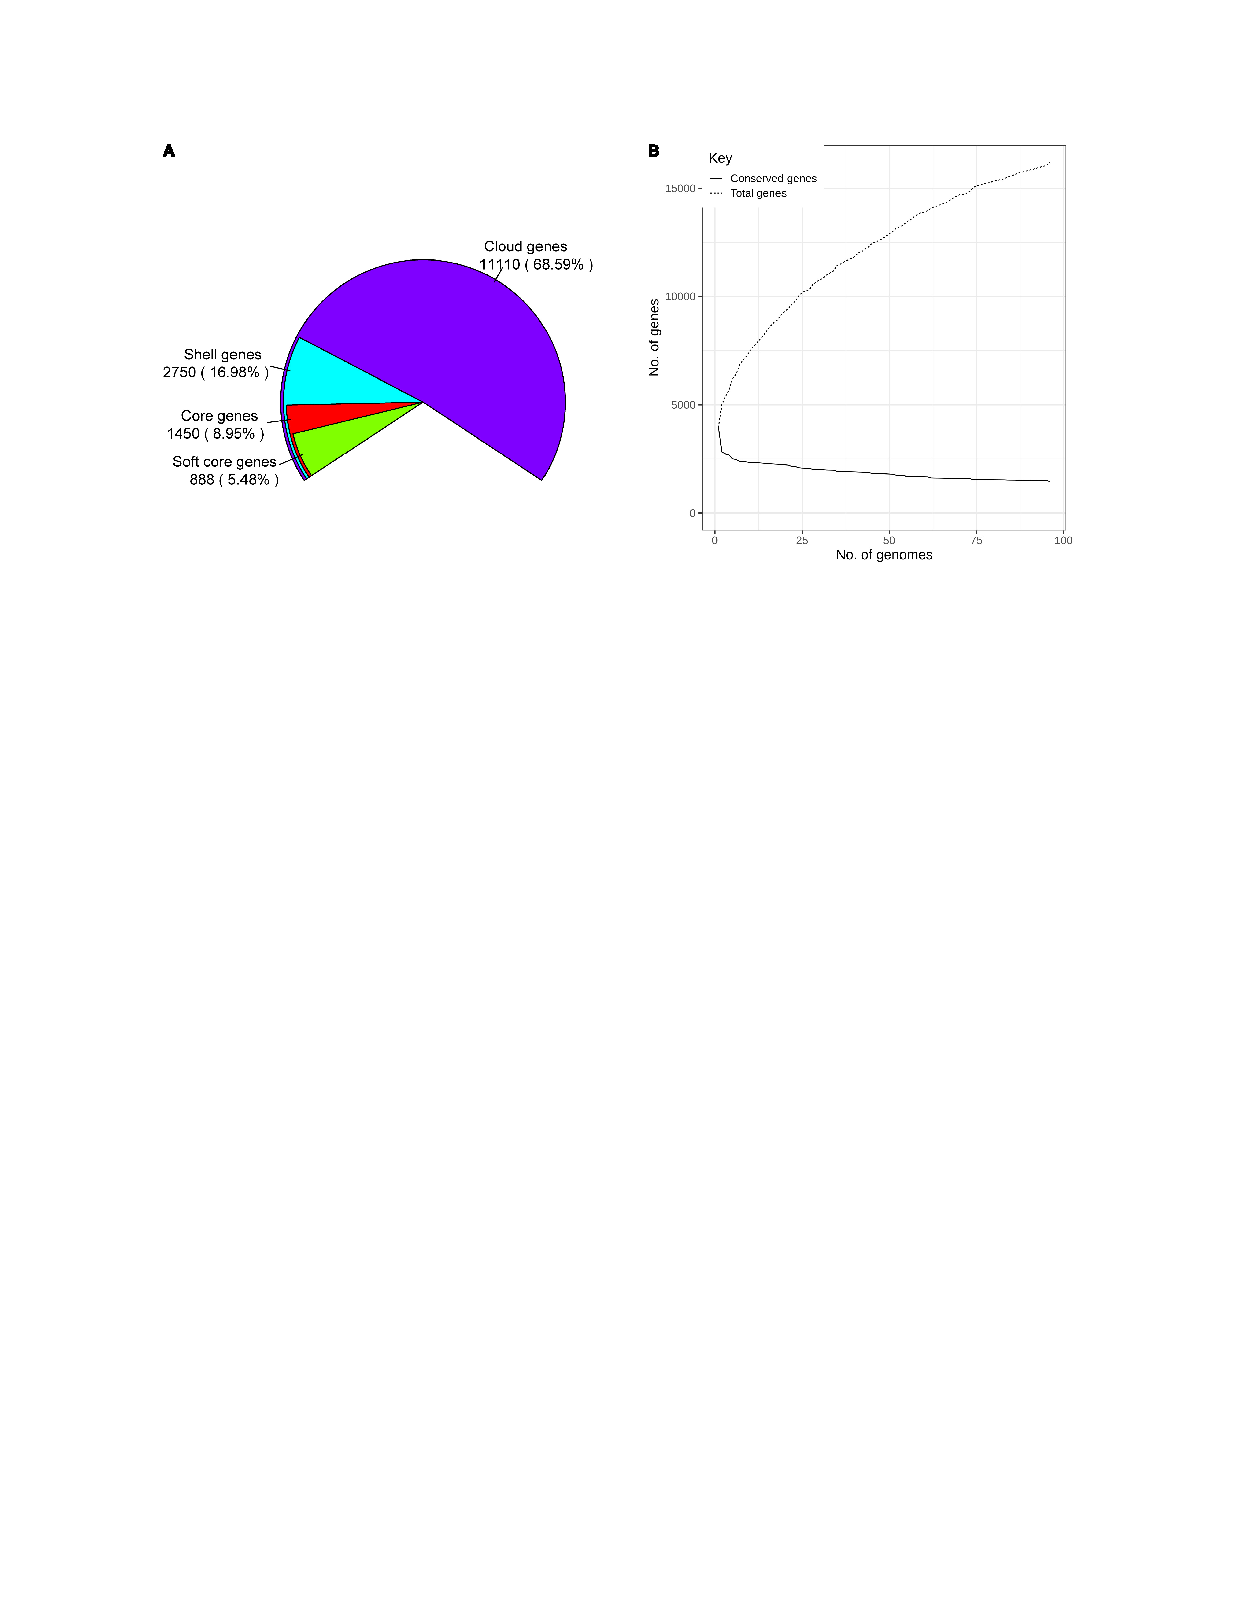
\includegraphics[width=\textwidth]{figures/figure1.pdf}
    \caption{96个解淀粉芽孢杆菌泛基因组。(A)基因的饼图分解(核心:$99\% \leq  菌株 \leq100\%,软核心:95\% \leq 菌株 < 99\%,壳层:15\% \leq 菌株 < 95\%,云层:0\% \leq 菌株 < 15\%$)。(B) 96 个基因组的泛基因组曲线。}
\end{figure}


通过构建基于1 154个串联核心蛋白序列比对的系统发育树(图2),研究了96个解淀粉芽孢杆菌菌株之间的进化关系。使用了短小芽胞杆菌SAFR-032(Gioia等人,2007)作为外类群。菌株分为两个支系,其中支系2包含两个簇。菌株分离的位置在系统发育树外以彩色条的形式进行了映射。来自美洲的菌株主要位于支系2的簇2中,而来自亚洲和欧洲的菌株分散在所有支系中。菌株的分离来源也在树上进行了标记。根据已知信息,几乎所有与植物相关的菌株都位于支系 2,而从食物中分离的菌株主要位于支系 1。上述结果表明解淀粉芽孢杆菌 主要分化为与植物相关和与食物相关的两类,这一点在支系中清晰地显示出来。然而,从水、土壤等环境中分离出的一些解淀粉芽孢杆菌物种分散在支系2中。

\begin{figure}[!htb]
    \centering
    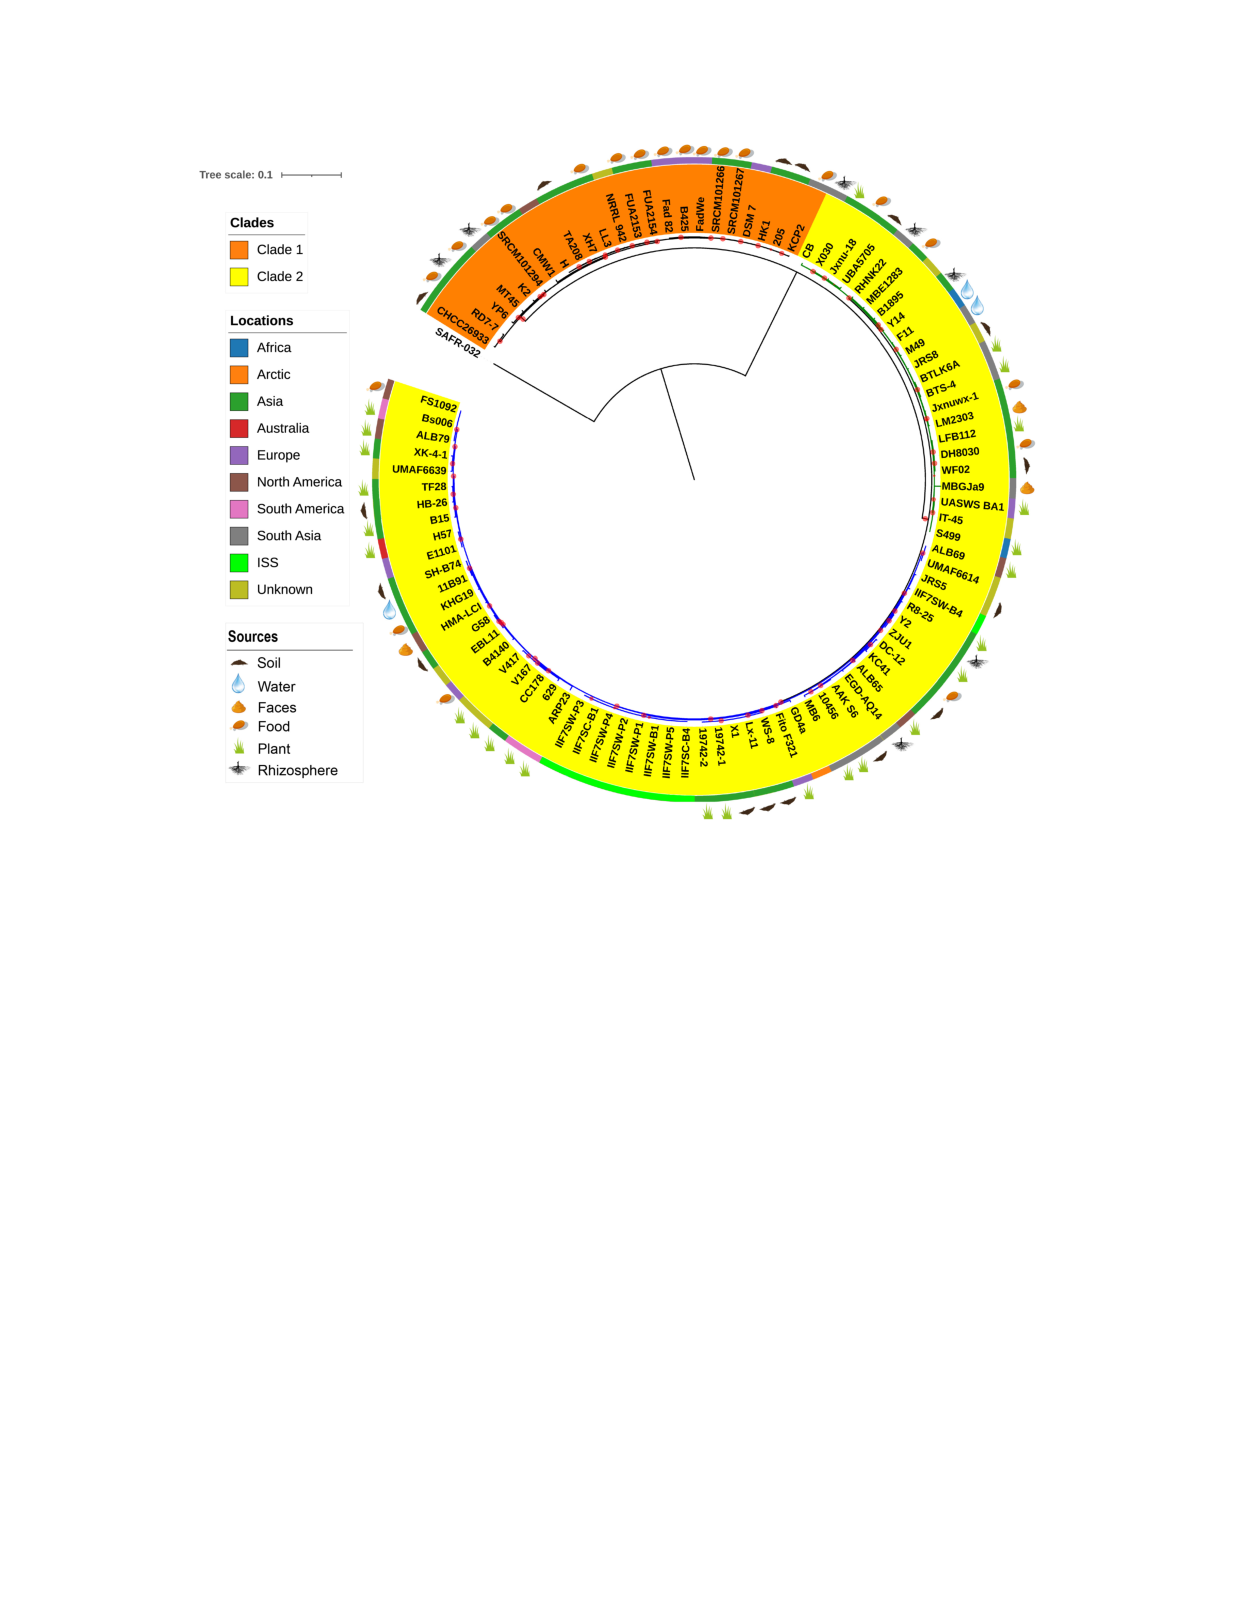
\includegraphics[width=\textwidth]{figures/figure2.pdf}
    \caption{单拷贝核心蛋白的系统发育树。使用 PGCGAP v1.0.21 的 ``CoreTree'' 模块构建的最大似然树(使用最佳拟合模型 JTT+F+R4)。树以 Bacillus pumilus SAFR-032 作为合适的外类群进行根植。树枝上的红圈代表大于 80\% 的 bootstrap 值。标签背景色(颜色范围)代表不同的支系,绿色和蓝色分支分别代表支系 2 中的簇 1 和簇 2。树外的彩色条描述了菌株的分离地点;ISS 代表国际空间站。树外的卡通图示表明菌株是从土壤、食物、根际、水或食草动物的面部分离的,或与植物相关联。}
\end{figure}

基因组对的相似性已在支系内部以及支系和簇之间进行了比较(图3)。发现支系1中的基因组比支系2中的基因组更相似($\mathrm{p < 0.001}$),而两个支系之间的基因组相似性非常低,这表明支系2 中的菌株经历了更多的分化,这可能与它们适应特定植物和其他相关生态位有关。当关注支系2时,簇1中的基因组比簇2中的基因组更相似($\mathrm{p < 0.001}$),而两个簇之间的基因组相似性相对较低。

\begin{figure}[!htb]
    \centering
    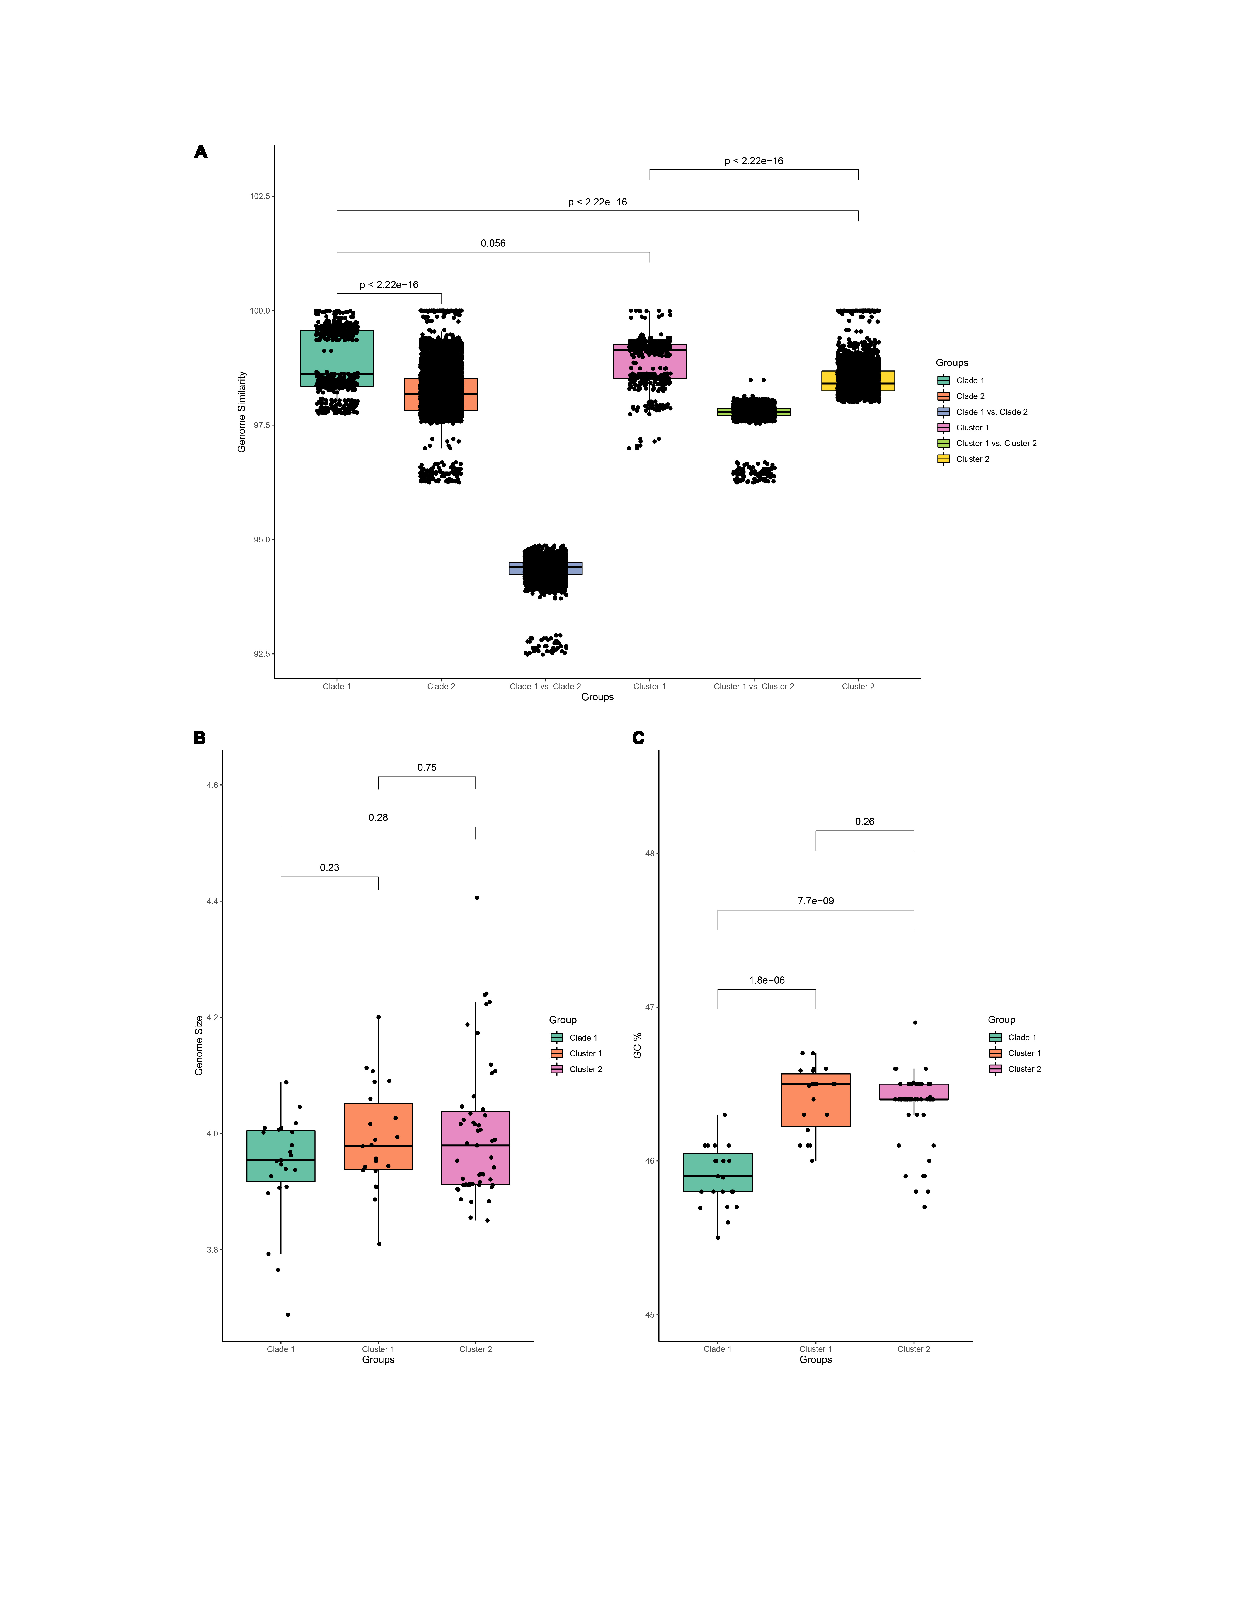
\includegraphics[width=\textwidth]{figures/figure3.pdf}
    \caption{解淀粉芽孢杆菌的基因组特征。(A) 支系 1 中所有菌株对之间的基因组相似性,支系 2 中所有菌株对之间的基因组相似性,支系 1 与支系 2 中菌株之间的基因组相似性,簇 1 中菌株对之间的基因组相似性,簇 2 中菌株对之间的基因组相似性,以及簇 1 与簇 2 中菌株之间的基因组相似性。(B) 支系 1 和簇 1 以及簇 2 的基因组大小。在箱形图顶部标记了 Wilcox 测试。(C) 支系 1、簇 1 和簇 2 的 GC 百分比。在箱形图顶部标记了 Wilcox 测试的 p 值。}
\end{figure}

与支系2的基因组相比,支系1的基因组具有独特的基因组成(图4A)。观察到支系1中的所有物种丢失了 335 个基因(补充表 2 第 2 592--2 926 行),这些基因存在于支系 2 的所有基因组中,并且拥有490独特的核心基因(补充表 2 第 3 969--4 458 行)。为了揭示两个支系之间的基因内容差异,使用了PGCGAP v1.0.21 的 ``OrthoF'' 模块进行了基因家族分析。共发现了 9 245 个正交群,其中 4 872 正交群在两个支系之间是共有的,而 1 055 个是支系 1 独有的,其余 3 363 个是支系 2 独有的。这些独正交群的功能通过 COG 注释揭示,如图 4B 所示。与支系 1 相比,支系 2 中功能类别 I(脂质转运和谢)、G(碳水化合物转运和代谢)和 Q(次级代谢物的生物合成、转运和分解)的相对丰度更高,而类别 D(胞周期控制、细胞分裂、染色体分离)、E(氨基酸转运和代谢)、H(辅酶转运和代谢)、L(复制、重组和复)、M(细胞壁 / 膜 / 包膜生物生成)和 X(移动组:噬菌体、转座子)的相对丰度在支系 1 中比支系 2高(图 4B)。
\begin{figure}[!htb]
    \centering
    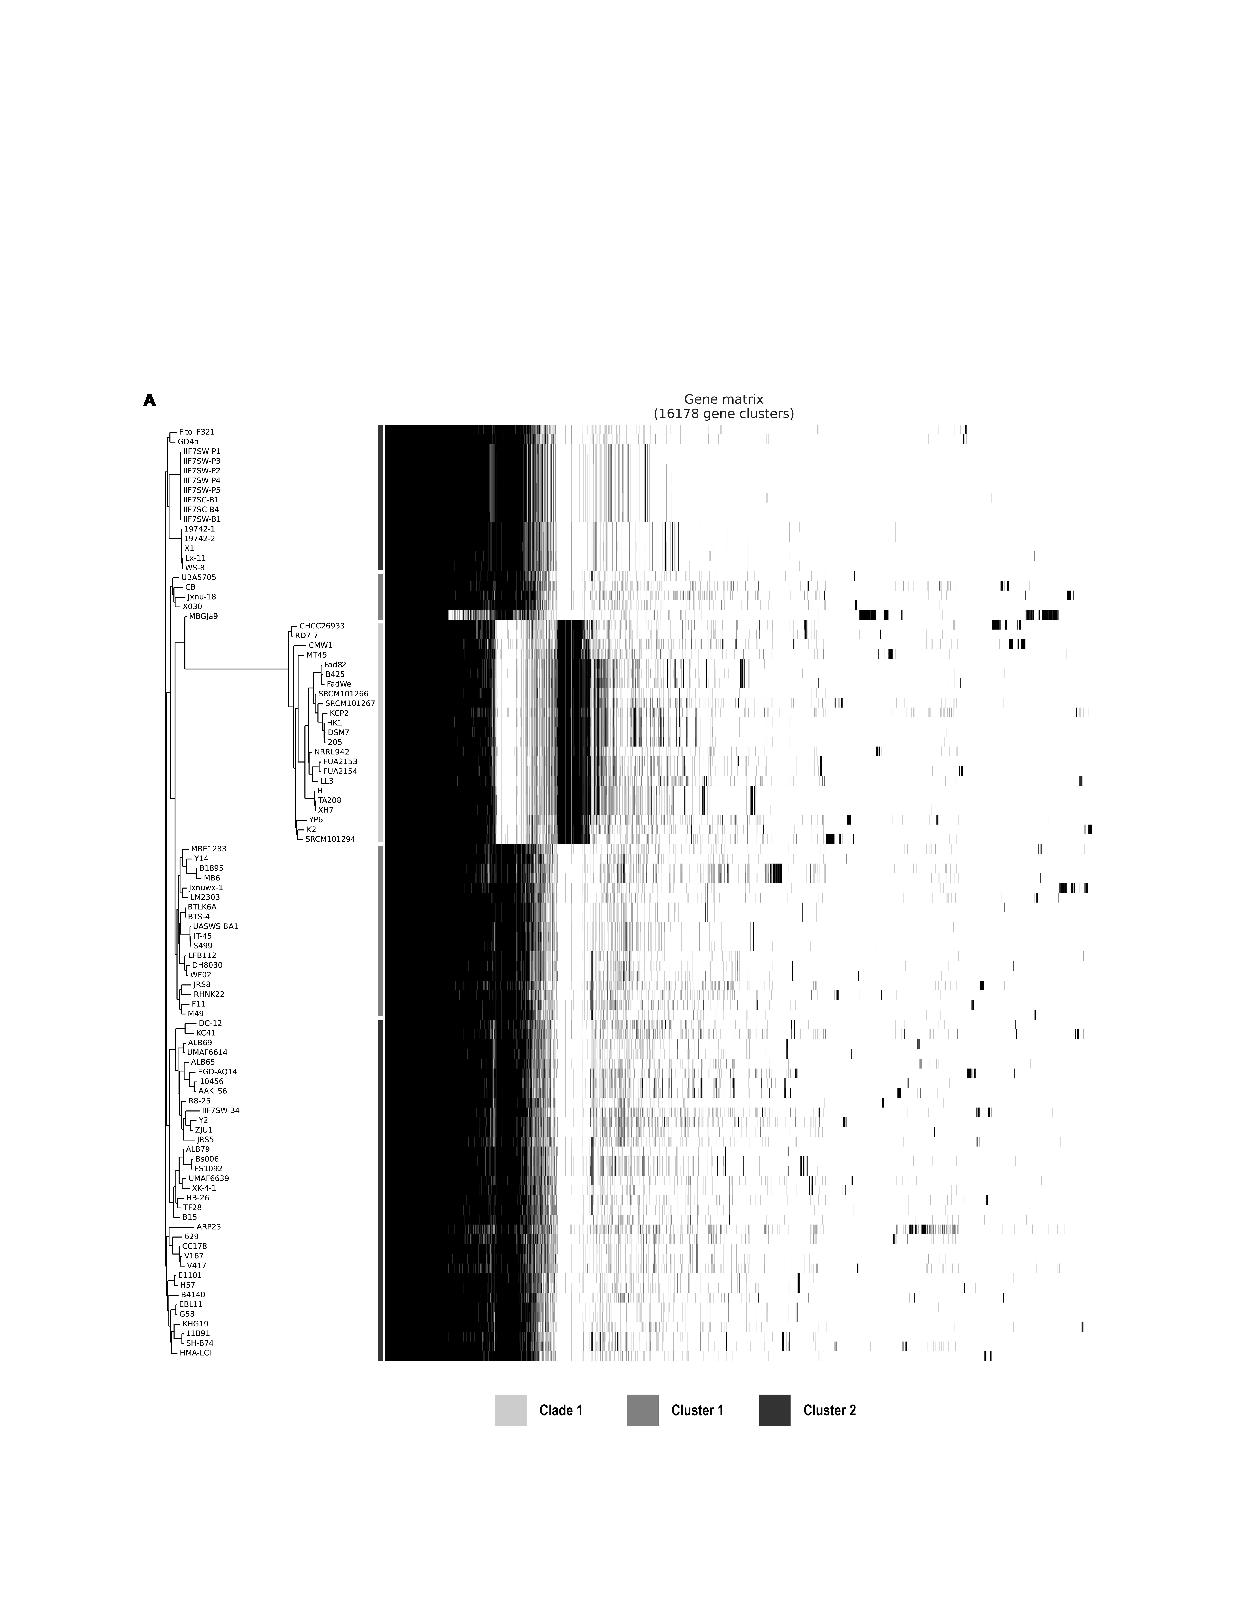
\includegraphics[width=\textwidth]{figures/figure4A.pdf}
    \caption{续}
\end{figure}

\begin{figure}[!htb]
    \addtocounter {figure}{-1}
    \centering
    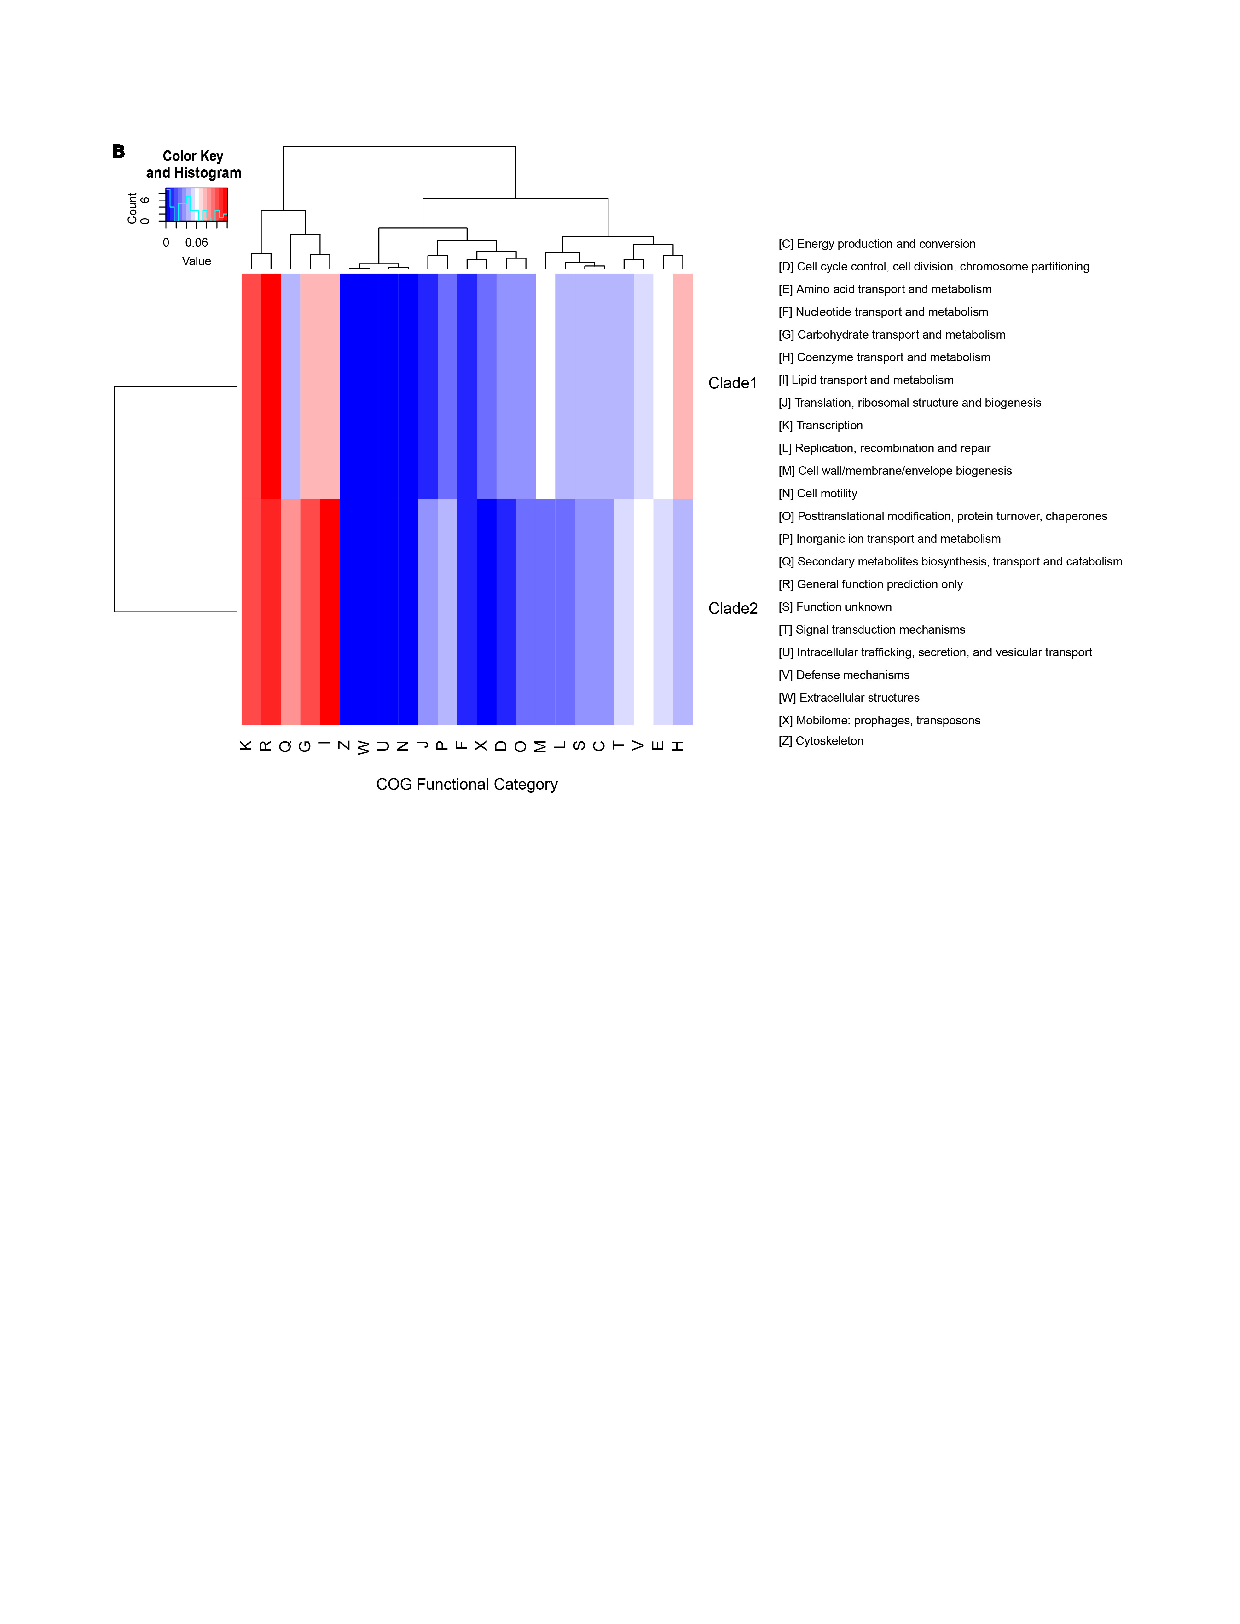
\includegraphics[width=\textwidth]{figures/figure4B.pdf}
    \caption{支系 1 和支系 2 之间的基因家族比较。图显示了树与存在和缺失核心和附属基因的矩阵的比较(A);树和矩阵之间的条形图显示了菌株属于哪个支系 / 簇。热图显示了对应于支系 1 和支系 2 的独特正交群的功能类别的相对丰度(B)。}
\end{figure}

众所周知,抗微生物耐药性和毒力基因根据各自生态位的功能在环境中传播;因此,我们调查了这些基因在解淀粉芽孢杆菌中的分布。来自不同数据库的抗微生物耐药性和毒力基因已被挖掘并映射在系统发育树上(图 5)。为了更清晰地展示树的拓扑结构,已移除外类群菌株,并将树以中点根的形式呈现。包括来自食物的所有解淀粉芽孢杆菌菌株都含有一个以上的毒力因子。观察到 $tmrB$ 和 $yuaB$ 仅存在于支系2 中,而 $clpP$ 仅在支系 1 中普遍存在。$tmrB$ 基因是一种在枯草芽孢杆菌中发现的与三磷酸腺苷结合的衣霉素抗性蛋白(Noda等人,1995),而 $yuaB$ 基因可以在枯草杆菌生物膜周围形成一层高度疏水层(Kobayashi和Iwano,2012)。基因 $clpP$ 编码一种参与蛋白水解的丝氨酸蛋白酶,并且在应激条件下生长是必需的(Gaillot 等人,2000, 2001)。有趣的是,解淀粉芽孢杆菌菌株 MBGJa9 比其他菌株拥有更多的毒力因子,并且可以看到 $isdA$、$isdB$、$isdC$、$isdD$、$isdE$、$isdF$、$isdG$ 和 $srtB$ 形成了一个基因簇,其产物参与了铁和血红素的摄取(Skaar 和 Schneewind,2004;Skaar 等2004)。

\begin{figure}[!htb]
    \centering
    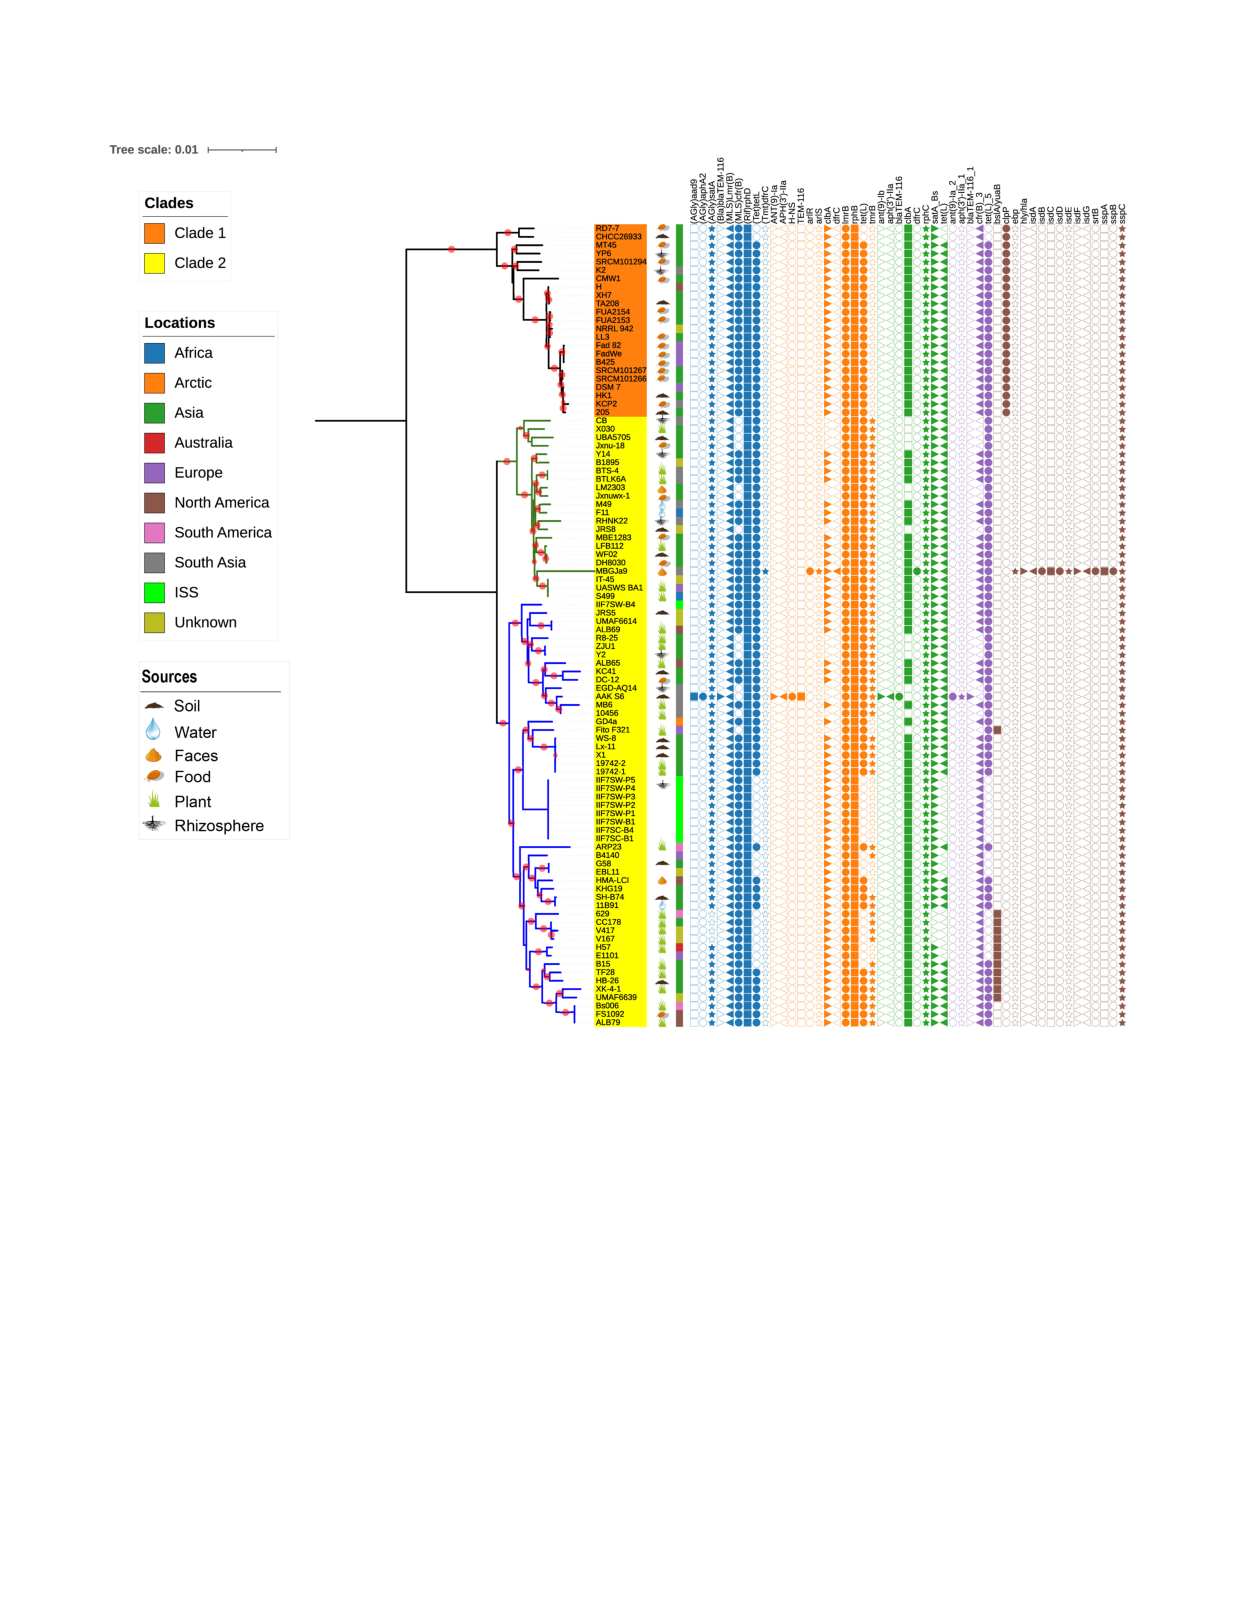
\includegraphics[width=\textwidth]{figures/figure5.pdf}
    \caption{单拷贝核心蛋白的中点根系统发育树。使用 PGCGAP v1.0.21 的 ``CoreTree'' 模块构建的树(使用最佳拟合模型 JTT+F+R4)。树枝上的红圈代表大于 80\% 的 bootstrap 值。标签背景色代表不同的支系,绿色和蓝色分支分别代表支系 2 中的簇 1 和簇 2。树后的菌株名称后的符号表示菌株是从土壤、食物、根际、水或食草动物的面部分离的,或与植物相关联。树外的彩色条描述了菌株的分离地点;ISS 代表国际空间站。树右侧的符号代表来自每个数据库的抗生素抗性基因或毒力基因 [蓝色:argannot (Gupta 等人,2014),橙色:card (Jia 等人,2017),绿色:NCBI (Michael Feldgarden 等人,2019),紫色:resfinder (Zankari 等人,2012),灰色:vfdb (Chen 等人,2016)]。}
\end{figure}


\section{讨论}
\subsection{解淀粉芽孢杆菌泛基因组评估}
目前对96株解淀粉芽孢杆菌的研究表明,它具有广泛的泛基因组,并且它代表了大量的基因,这些基因被观察到与每个不同的物种唯一相关。解淀粉芽孢杆菌的种群规模和相应的生态位多样性被认为是决定泛基因组大小的最有影响力因素,可以看到相对于基因组序列总数的总基因数正在上升,因此无法想象完整泛基因组的大小。由于分离来源和地理位置,淀粉芽孢杆菌的开放泛基因组并不令人惊讶,这些因素总是为物种的整体基因库添加新基因。这种物种分化可能是不同机制(如水平转移、转座和转化)的属性(Konstantinidis 和 Tiedje,2005; Tettelin 等人,2005)。相反,调查中观察到的核心基因数量较少,可能是由于基因组数量较多、其他属的基因组的整合,以及数据集中包括草图基因组(Lefebure 等人,2010; Inglin 等人,2018)。众所周知,不完整、未完成或部分组装的基因组对分析中核心基因组的出现有很大的影响,因为核心基因组似乎对异质数据集和质量差的序列非常敏感(Mendes-Soares 等人,2014)。

\subsection{基于单拷贝核心蛋白和基因组比较的解淀粉芽孢杆菌系统进化分析}

16s rRNA 已被广泛用于原核生物的分类评估,并作为广泛背景,尽管通过``多相方法'' 实现微生物物种的更好分类分辨率是非常有效的(Rosselló-Mora 和 Amann,2001; Na 等人,2018)。16s rRNA 的存在限制了物种或亚种水平的基因组分辨率,因此强烈建议将基因组序列应用于对微生物物种的分类学理解,而不是常规使用的DNA-DNA杂交和16 s rRNA基因组学(Chun et al,2018)。因此,与其使用单个基因,基于基因组的系统发育,称为系统基因组学,已经建立了更好的分类定位,因为它使用一组核心基因(Eisen 和 Fraser,2003)。所有解淀粉芽孢杆菌菌株的基因组序列都可以在 NCBI 基因库数据库中获得,这使我们能够确定所有物种之间的基因组变异程度,以及区分所有分离株的分类有效性,并重建它们的系统发育关系。当使用单拷贝核心蛋白推断系统发育时,观察到两个不同的支系。支系 1 包括 23 个 解淀粉芽孢杆菌 菌株,其中 56\% 与食物相关,17.39\% 来自土壤,8.69\% 是根际的。支系 2 包括 73 个菌株,它被区分为两个不同的簇,其中簇 1 和簇 2 分别包含 22 个和 51 个 解淀粉芽孢杆菌 菌株。支系 2 在植物起源宿主 / 宿主的物种中更为丰富,约占 35.61\%,而土壤、食物、室内生物群落和根际来源的菌株分别为 16.43\%、10.95\%、12.32\% 和 6.84\%。划分了两个不同的支系,其中一个与食物相关(支系 1),另一个与植物相关(支系 2)。核心基因集的选择用于准确的系统发育分析可能会随着分析时基因组序列的可用性而有所不同。

两个支系菌株之间的基因组相似性比较表明,支系 1 中分组在一起的菌株比支系 2 中的菌株更相似。解淀粉解淀粉芽孢杆菌的大多数与植物相关的菌株被归类在进化枝2下,而非与植物相关的菌株主要被发现在进化枝1中,尽管相对于一些其他生态位看到一些分散。与植物相关的 解淀粉芽孢杆菌 菌株在其基因组中采用了更多的修改,这直接关系到它们对特定植物的适应。因此,人们相信与植物相关的 解淀粉芽孢杆菌 菌株的基因组大小总是大于非植物相关 解淀粉芽孢杆菌 的基因组大小,以及 GC 含量。Zhang N.等人(2016)报道了解淀粉解淀粉芽孢杆菌植物相关菌株的核心基因组中,与非植物相关菌株相比,具有更多的中间代谢和次生代谢产物生物合成相关基因,植物相关菌株还具有合成抗生素和利用植物源底物的特异基因。

在评估核心和附属基因时,观察到支系 1 中的 解淀粉芽孢杆菌 菌株丢失了许多存在于支系 2 菌株中的基因(图 4A)。外多糖(EPSs)在细菌中扮演非常重要的角色,特别是那些与植物相关的细菌,具有多种功能。它帮助微生物在粘附、致病和共生中发挥作用,以及在一些不利条件下保护免受干燥(Stingele 等人,1999)。糖基转移酶基因区域包括 EPS 基因簇,即 $epsF-2$、$epsD$、$epsI$、$epsM$、$epsL$ 和 $epsJ$,这些基因参与 EPS 的生物合成,在与植物相关的 解淀粉芽孢杆菌 菌株中具有深远的作用,而在属于支系 1 的菌株中缺失。与植物相关的 解淀粉芽孢杆菌 菌株(支系 2)携带一个在支系 1 中缺失的特定基因簇,该基因簇通过非核糖体肽合成酶(NRPS)包括 fengycin($fen$)参与脂肽的生物合成。参与 bacillaene($bae$)合成的基因簇负责强烈的抗微生物活性,并在支系 1 中的所有 解淀粉芽孢杆菌 菌株中丢失。PKS 基因簇,包括 $pksI\_2$、$pksG\_2$、$pksN\_2$ 和 $pksS$,也被发现存在于支系 2 中,但在支系 1 中丢失(图 4A)。一些基因,如胱硫醚 $\beta$- 裂解酶(patB)、假定的多药耐药 ABC 转运蛋白 ATP 结合 / 渗透酶蛋白(yheI)、冷休克蛋白(cspC)、精胺 / 精胺 N (1)-乙酰转移酶(paiA)、假定的糖磷酸异构酶(ywlF)、3 - 脱氢石酸脱水酶(asbF)、假定的 ABC 转运蛋白底物结合脂蛋白(yhfQ)、亚铁螯合酶(sirB)、假定的金属水解酶(yflN)、二肽基肽酶 5(ddp5)、L - 天冬氨酸氧化酶(nadB)、假定的孢子形成水解酶(cotR)、应激反应激酶 A(srkA)、Sortase D(srtD)、ATP 依赖的脱硫生物素合成酶(bioD 1)、甘油磷酸二酯磷酸二酯酶(glypQ)、叶酸多谷氨酸合成酶(fpgS)和假定的 ABC 转运蛋白渗透酶(ytrC)被发现独特地与属于支系 1 的 解淀粉芽孢杆菌 菌株相关联。因此,支系 2 中某些基因簇的存在和支系 1 中的缺失得出结论,与非植物相关菌株相比,与植物相关的 解淀粉芽孢杆菌 菌株具有更丰富的中间代谢以及抗生素生产的基因簇。Niazi等人2014)报道了解淀粉芽孢杆菌植物亚种($B.~amyloliquefaciens$~subsp.~$plantarum$),一种修复植物生长和胁迫管理的根际细菌,也具有更丰富的基因簇,其积极参与某些水解酶以及次级代谢产物的产生。众所周知,由于根分泌物的影响以及微生物之间的持续互动和竞争,根际环境拥有一个非常动态的微生物群落,它们需要相互竞争各种资源,如营养供应,这最终导致它们产生各种代谢物,如抗生素和胞外水解酶(Bais 等人,2006)。

\subsection{淀粉芽孢杆菌所有菌株中耐药性和毒力基因的监测}

据记载,细菌产生抗生素已有数百万年的历史,这导致了耐药基因的进化和诱导。更确切地说,抗生素在农业和某些工业应用中的密集非医疗用途并不确定,并导致了耐药基因在环境中的大量传播(Pawlowski et al,2018)。 将所有解淀粉芽孢杆菌菌株的基因组定位到不同的数据库中,以评估抗生素抗性基因和毒力基因的分布,发现许多不同的基因分散在所有解淀粉芽孢杆菌菌株中;此外,所观察到的基因属于多种抗性类别。基因(AGlu)$satA$编码酶氨基糖苷乙酰转移酶,属于氨基糖苷类,几乎存在于所有菌株中,与其宿主环境无关。氨基糖苷类被认为是广谱抗生素的一部分,通过抑制蛋白质合成发挥作用,但与其他抗菌剂协同作用最佳(Krause et al,2016)。 在研究中考虑的大多数菌株中存在属于大环内酯类林可酰胺-链阳性菌素B(MLS)的两种基因$lmrB$和$cfrB$,$lmrB$和$cfrB$的基因产物分别赋予对林可酰胺类(如林可霉素和克林霉素)和合成抗生素利奈唑胺的特异性耐药性(Kim et al,2001; Toh et al,2007)。新的、更稳定的大环内酯类抗生素的出现及其不明确的使用可能是诱导这些抗性赋予基因的关键原因,并且它为微生物种群获得MLS抗性提供了机会(Roberts等,1999)。(Rif)$rphD$、$rphB$和$rphC$基因编码三氟霉素激酶(磷酸转移酶),它赋予对利福平的抗性,利福平是最常用的利福霉素。利福平磷酸转移酶存在于许多环境细菌中,这一现象过去是由选择性压力和非临床使用抗生素引起的,导致利福平和ATP失活为磷酸化利福平和AMP+Pi(Stogios等人,(2016年)在农业和工业用途的许多细菌属中已经报道了超过40种不同的四环素抗性基因。在细菌属中tetL基因比任何其它tet抗性基因高得多(Roberts,2005)。在本研究中,所有菌株的基因组序列在argannot、NCBI、plasmidfinder、card、resfinder和yfdb等6个不同的数据库中进行了定位,结果表明所有菌株都存在$tetL$基因。大肠杆菌素是许多肠道细菌中由$clb$基因簇编码的遗传毒性分子,在自然界中广泛分布(Kawanishi等,2020)。$clbA$ 是一种质粒编码的 $cfr$ 基因,其受到 $B.~velezensis$($B.~amyloliquefaciens$ subsp. $plantarum$)中报告的可诱导启动子的控制,而 $clbB$ 和 $clbC$ 分别存在于 $Brevibacillus~brevis$ 和 $B.~clausii$ 中(Hansen 等人,2012 年)。基因$sspC$编码称为葡萄球菌蛋白酶抑制素的细胞质蛋白,并且存在于解淀粉芽孢杆菌的所有菌株中。它是葡萄球菌蛋白酶B(Ssp B)的特异且紧密结合的抑制剂。 sspC的主要功能是保护胞浆蛋白免受错误折叠或激活的SspB的降解。 Shaw等(2005)报道,在缺少sspC蛋白的情况下,细胞生理学发生重大改变,微生物细胞的生长和活力受损。编码酪蛋白分解蛋白酶蛋白水解亚基(ClpP)ClpP蛋白赋予微生物在不同的环境条件以及胁迫条件下维持的某些优势。ClpC和ClpP是热休克蛋白,并且是ATP的亚基。解淀粉芽孢杆菌中报道的依赖性蛋白酶。$clpC$和$clpP$基因的转录在非胁迫条件下始终受到负调控(Krüger等,2001)。由于ClpP蛋白功能的改变,许多微生物/病原体的毒力和感染性受到影响。Clp蛋白是高度保守的,并且在原核细胞和真核细胞器的蛋白水解中起着非常重要的作用,尽管只有少数报告描述了Clp介导的蛋白水解在生物体中的重要性(Krüger等人,2001; Moreno-Cinos等人,2019)。 衣霉素是一种核苷类抗生素,能杀死大多数革兰氏阳性菌,它通过抑制细胞壁中的磷壁酸来发挥作用,磷壁酸是微生物生理和致病的重要组成部分,在衣霉素的亚抑菌浓度下,细菌的生物被膜生成减少,毒力蛋白减少,细菌的粘附和侵袭能力降低(Zhu et al,2018)。$tmrB$基因的存在导致TmrB蛋白的产生,其赋予枯草芽孢杆菌衣霉素抗性。TmrB蛋白存在于细胞质和膜部分中,尽管它完全是亲水性的,但它通过其C端的两亲性$\alpha$螺旋附着在膜上(Noda等人,1995)。许多植物生长促进细菌产生生物膜,这是它们在某些恶劣条件下以及在植物根际环境中成功生存的关键策略。 微生物的生物膜形成能力使其成为良好的生物防治剂,因为它导致真菌和细菌病原体引起的感染减少(Hobley等人,2013)。 解淀粉芽孢杆菌的许多植物相关菌株中存在的$bslA$/$yuaB$基因编码独特的表面活性蛋白BslA,其形成称为疏水蛋白的疏水表面层。表面层调节各种分子的扩散、来自其他微生物群落的信号分子的感知以及营养吸收,生态和进化事实的背景信息以及比较基因组学的应用和基因组测序成本的下降共同有助于更精确地理解微生物多样性的结构,系统发育学揭示了所有96株解淀粉芽孢杆菌分为两个分支。大多数与植物相关的解淀粉芽孢杆菌菌株被聚在分支2中,而分支1主要是与食物相关的菌株。所有解淀粉芽孢杆菌菌株中的抗性和毒力基因的分布已经报道,它将作为一个基准和资源丰富的信息,以推断假设或结论,以及开发潜力的任何菌株通过湿实验室实验。在未来的招股说明书,我们将试图挖掘出一些时间基因及其发生模式,以了解微生物的重要作用以及整个微生物群落的结构各自的生态位。

% \includepdfmerge{trans_ref_thesis.pdf,1-12}
\end{document}